5つの幅があり,各自の幅で各十回(毎回8分間)実験する,毎回の実験で,ランダムでロボットを2つグループを分ける.$T_{\rm sd}$と流量の平均値と分散を計測する
\begin{table}[!ht]
\begin{center}
\begin{tabular}{|c|c|c|c|c|}
\hline
幅 & $T_{\rm sd}$(秒) & $T_{\rm sd}$ & 流量 & 流量 \\
($cm$)   &   平均値 & 分散 & 平均値 & 分散 \\
\hline
43 & 0 & 0 & 0 & 0 \\
\hline
49.5 & 0 & 0 & 0 & 0 \\
\hline
56 & 277.8 & 17838.56 & 2.345 & 33.558 \\
\hline
62.5 & 274.1 & 11389.69 & -0.354 & 18.399 \\
\hline
69 & 273.4 & 19343.84 & 0.118 & 41.541 \\
\hline
\end{tabular}
\end{center}
\caption{
幅により$T_{\rm sd}$と流量の値
}
\end{table}

\begin{figure}[ht]
    \centering
    \includegraphics[width=1.0\linewidth]{diagram3.png}
    \caption{}
\end{figure}
\begin{figure}[ht]
    \centering
    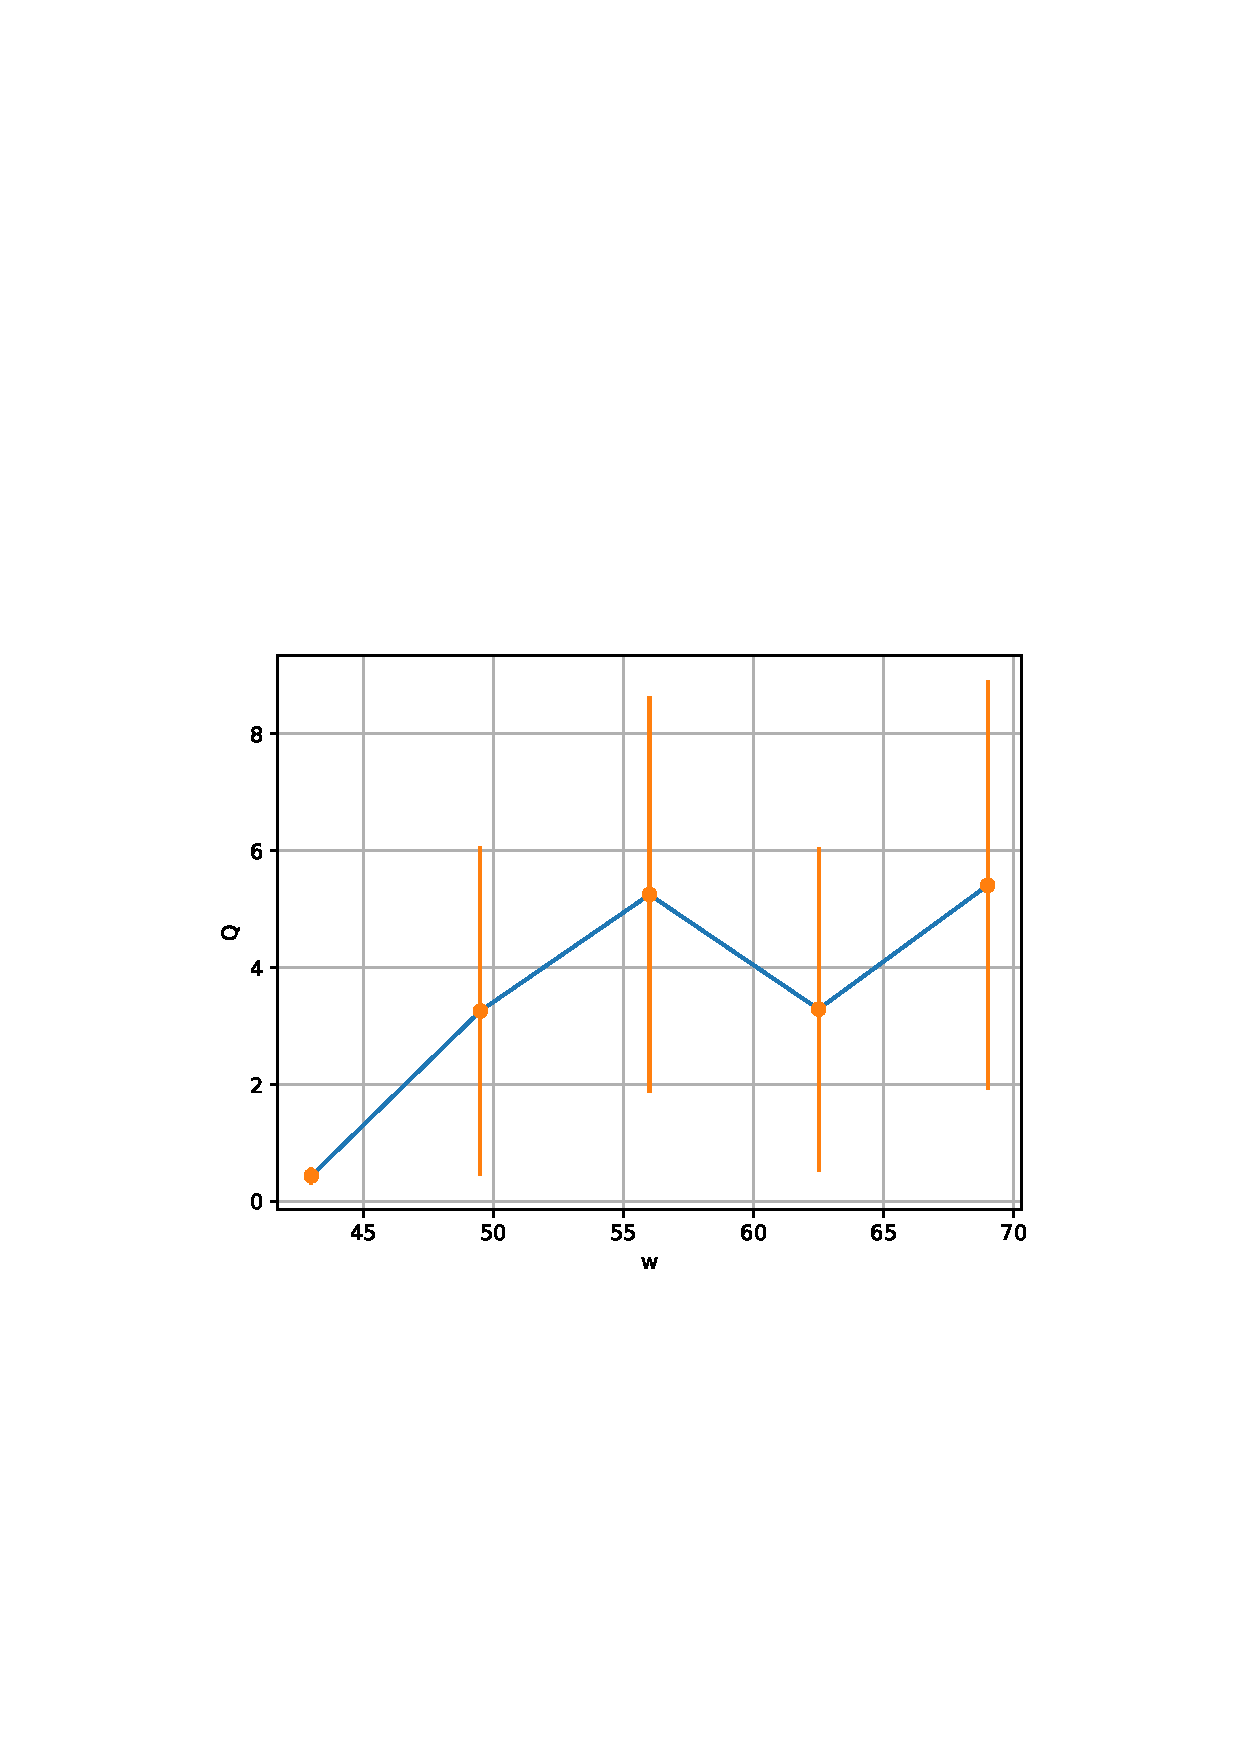
\includegraphics[width=1.0\linewidth]{diagram4.png}
    \caption{}
\end{figure}

図$7$が幅の拡大に従って,$T_{\rm sd}$の変化曲線である.図$8$が幅の拡大に従って,流量($Q$)の変化曲線である.
幅が狭すぎる(43$cm$)と,長時間の渋滞が発生したことを観測した,ロボット同士が互いに引っかかって,方向転換もできなくて,one direction flow の状態も出なかった.大渋滞ので,流量もほとんどない.49.5$cm$の場合,渋滞も起こったので,one direction flow 状態になる時間($T_{\rm sd}$)も長かった,ロボットがギリギリ方向転換できて,流量もふえてきた.56$cm$から渋滞がほとんどなくて,ロボットの方向転換もしやすくなって,$T_{\rm sd}$が急激に減少して,幅がもっと広まっても,あんまり変わらないようになった.それに,幅が広まっていって,右回りと左回りのロボットの数が相当で,対面走行ができて,流量も減少していった(完璧な対面走行の流量が$0$である)

